\documentclass[12pt]{report}

\usepackage{commands}


\begin{document}

\large

\begin{center}
 Math 568 Homework 6\\
 Due February 21\\
 By Marvyn Bailly\\
\end{center}

\normalsize

\hrule

%---------------%
%---Problem 1---%
%---------------%

%--status--$

\begin{problem}
    Consider the singular equation:
    \[ 
        \eps y'' + (1+x)^2y' + y = 0,
    \]
    with $y(0) = y(1) = 1$ and with $0< \eps \ll 1.$
    \begin{enumerate}
        \item [(a)] Obtain the leading order uniform solution using the WKB method. 
        \item [(b)] Plot the uniform solution for $\eps = 0.01, 0.05, 0.1, 0.2$. 
    \end{enumerate}

\end{problem}

\begin{solution}

    \noindent
    Consider the singular equation:
    \[ 
        \eps y'' + (1+x)^2y' + y = 0,
    \]
    with $y(0) = y(1) = 1$ and with $0< \eps \ll 1.$

    \begin{enumerate}
        \item [(a)]
        We wish to obtain the leading order uniform solution using the WKB method. We begin by assuming the solution takes the form
        \[ 
            y(x) = \text{exp} \paren{ \frac{S_0(x) + \eps S_1(x) + \eps^2 S_2(x) + \cdots}{\eps} }.
        \]
        Inserting this ansatz into the governing equation, collecting terms and dividing out the expontial yields
        \begin{align*}
            \O(e^{-1}):& ~~~ S_{0_x}^2 + (1 + x)^2S_{0_x} = 0,\\
            \O(e^{0}):& ~~~ S_{0_{xx}} + 2S_{0_x}S_{1_x} + (1  + x)^2S_{1_{x}} + 1 = 0.
        \end{align*}
        The leading order problem can be rewritten as
        \[ 
            S_{0_x} \paren{S_{0_x} + (1 + x)^2} = 0,
        \]
        which gives the two solutions $S_{0_x} = 0$ or $S_{0_x} = - (1 + x)^2$. 

        \noindent
        In the case when $S_{0_x} = 0$, then $S_0$ is a constant. Plugging this result into the $O(1)$ equation gives
        \[ 
            S_{1_x}(1 + x)^2 + 1 = 0,
        \]
        and solving for $S_1$ gives
        \[ 
            S_1 = - \int_0^x \frac{1}{(1+\xi)^2} \dt{\xi} = \frac{1}{1 + x}.
        \]
        The WKB solution in this case is given by
        \[ 
            y(x) = \text{exp}\paren{\frac{S_0}{\eps} + S_1} = \text{exp} \paren{\frac{S_0}{\eps}}\text{exp}\paren{\frac{1}{1 + x}} = C_1 e^{\frac{1}{1 + x}}.
        \]

        \noindent
        Next consider when $S_{0_x} = - (1 + x)^2$. Plugging this into the $O(1)$ equation gives
        \[ 
            - (x+1)^2S_{1_x} -2 x = 1,
        \]
        and solving for $S_1$ gives
        \[ 
            S_1 = \int_0^x \frac{1}{(1 + \xi)^2} \dt{\xi} - \ln[(1 + x)^2] = -\frac{1}{1+x} - \ln[(1 + x)^2].
        \]
        Note that
        \[ 
            S_0 = -x - x^2 - \frac{x^3}{3}
        \]
        The WKB solution in this case is given by
        \begin{align*}
            y(x) &= \text{exp}\paren{\frac{S_0}{\eps} + S_1}\\
            &= \text{exp}\paren{\frac{1}{\eps}\paren{-x - x^2 - \frac{x^3}{3}} -\frac{1}{1+x} - \ln[(1 + x)^2]}\\
            &= \frac{C_2}{(1+x)^2}\text{exp}\paren{\frac{1}{\eps}\paren{-x - x^2 - \frac{x^3}{3}} -\frac{1}{1+x}}.
        \end{align*}

        This gives the solution
        \[ 
            y(x) = C_1 \text{exp}\paren{\frac{1}{1 + x}} + \frac{C_2}{(1+x)^2}\text{exp}\paren{\frac{1}{\eps}\paren{-x - x^2 - \frac{x^3}{3}} -\frac{1}{1+x}},
        \]
        and enforcing the initial conditions $y_1(0) = y_1(1) = 1$ we find that
        \[ 
            C_1 = -\frac{4 e^{\frac{7}{3 \epsilon }+\frac{1}{2}}-e}{e \left(e-4 e^{\frac{7}{3 \epsilon }}\right)},
        \]
        and
        \[ 
            C_2 = -\frac{4 \left(\sqrt{e}-1\right) e^{\frac{7}{3 \epsilon }+1}}{4 e^{\frac{7}{3 \epsilon }}-e}.
        \]
        Thus the uniform solution using the WKB method is given by
        \[ 
            y(x) = -\frac{4 \left(\sqrt{e}-1\right) e^{\frac{-\frac{x^3}{3}-x^2-x}{\epsilon }-\frac{1}{x+1}+\frac{7}{3 \epsilon }+1}}{(x+1)^2 \left(4 e^{\frac{7}{3 \epsilon }}-e\right)}-\frac{e^{\frac{1}{x+1}-1} \left(4 e^{\frac{7}{3 \epsilon }+\frac{1}{2}}-e\right)}{e-4 e^{\frac{7}{3 \epsilon }}}
        \]

        \item [(b)]
        Using Mathematica we can plot the uniform solution for $\eps = 0.01,0.05,0.1,0.2$ which gives the following figure.
        \begin{center}
            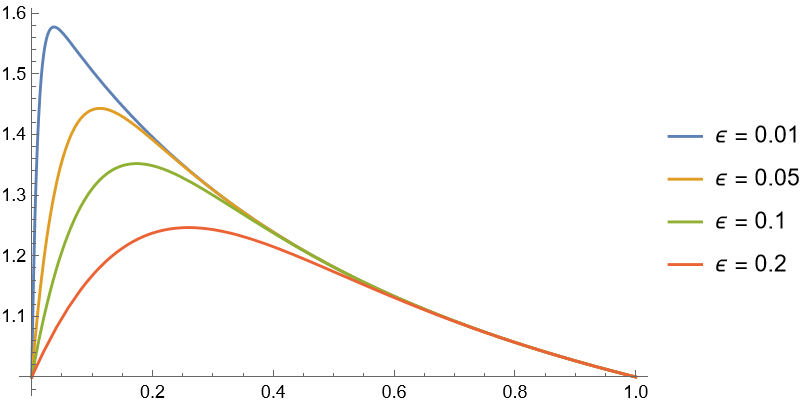
\includegraphics[width=.8\textwidth]{1.png}
        \end{center}
        
        
    \end{enumerate}
\end{solution}

%----------------------------------------------------------------------------------------------------%
%\vskip 20pt
\newpage


\end{document}